\documentclass{article}

\title{CS1102 Practical 1 Report}
\date{21/02/2018}
\author{150008859}

\setlength{\parskip}{1em}
\setlength{\parindent}{0em}

\usepackage{listings}
\usepackage{amsmath,amssymb,amsthm}
\usepackage{mathtools}
\usepackage{graphicx}
\usepackage{subfig}

\begin{document}
\maketitle
\newpage

\section{Introduction}

The aim of this practical was produce an efficient file replication scheme. In this practical, I was inspired by bittorent and implemented a P2P file sharing protocol along with an implementation of the Kademlia distributed hashtable for trackerless torrents.

\section{Usage}

This is an eclipse project. The bootstrapping node, download directory and torrents directory must be set in Config.java.

\begin{lstlisting}[language=bash]
  cd networking
  java -cp bin networking.torrent.client.TorrentService
\end{lstlisting}


\section{Kademlia}

To support trackerless p2p file sharing, I implemented the Kademlia distributed hash table the parameters of which are configurable in ``Config.java''.

\subsection{Node}

In my implementation, a node consists of an 8 bit key as the node's identification number, its ip address and port. 

\subsection{Distance Function}

The unsigned integer value of the xor metric is used to calculate the distance between two Kademlia nodes.

\subsection{Buckets}

The Kademlia buckets are a list of buckets storing Kademlia nodes. The number of buckets equals the quantity of bits in a key. There are 8 buckets present in my implementation storing up to 20 entries in linked lists.

Given our node and a node to be inserted, the number of bits the prefix differs by determines which bucket the node will be inserted in. Nodes which are furtheraway are stored in higher numbered buckets. 

A least recently seen scheme is used for node eviction.

The Kademlia buckets forms the routing table and can also used to retrieve the nodes closest to a given target.

The buckets are kept updated through the regular flow of traffic either from a querying node or from the nodes present in responses.

\subsection{Protocol}

The protocol is represented by Serializable Objects over udp. There is an object for each remote procedure call and its response.

The remote procedure calls include \textbf{ping}, \textbf{find node}, \textbf{fetch} and \textbf{store}.

A \textbf{ping} checks if a node is online, a \textbf{pong} message is sent in response.

A \textbf{find node} takes a key target rpc returns the closest k nodes to the given target.

A \textbf{fetch} rpc takes a key target and returns the target value or the k closest nodes if it doesn't have the value.

A \textbf{store} rpc is used to store a key value pair on a node.

\subsection{Tasks}

For each rpc, a task exists that uses the remote procedure calls.

A find node task will iteratively query the closest nodes it has knowledge of and query them with a find node rpc until it cannot find a node any closer.

A fetch task will iteratively query the closest nodes it has knowledge of and query them. If they return the key value pair, the search will be over. Otherwise, it will add the nodes returned by rpc to its pool of nodes.

A store task will use a find node task to obtain the closest nodes to a target key and send a store rpc.

\subsection{Concurrency}

For each Query, a BlockingQueue is created inside a Callable, the Callable polls the queue for the response with a timeout. This Callable is ran through an ExecutorService. The time that a query was generated at is used as a unique identifier. This identifier is mirrored in the response and maps it to the BlockingQueue the Callable is waiting on. The listener thread inserts the message into the BlockingQueue. In the Callable, this message is now available. 

A system wide parameter alpha is used to limit the number of asynchronous queries made. I have set alpha to the recommended value 3.

The ExecutorService accepts the callable objects and make the queries asynchronously returning Future Objects which can be polled. In my implementation, I use Java 8's functional programming interface to map the future's into a list of responses which is used by the task for the next iterative step.

\subsection{Bootstrapping}

Knowledge of atleast a node is required to join an existing network. The node joining node adds the given node to its buckets and issues a find node task with itself as the target.

\section{P2P File Sharing Protocol}

An important distinction to be made at this point that peers and nodes are different. A peer participates through file sharing over the p2p file sharing protocol, where as the node represents a Kademlia node which communicates with other Kademlia nodes via the Kademlia protocol and form the Overlay network.

\subsection{Torrent Files}

A torrent file represents the meta data of a file, it is a serializable object which stores the name, size and the list of all the SHA-1 hashes of pieces in a file. The torrent does not contain any of the content of the file itself.

A peer will automatically construct a torrent file for any present files in its download folder, this is available to all peers due to the nature of the lab's nfs. Alternatively, the user can also distribute this torrent file.

The torrent file is used by peers contains all the data required to reconstruct the original file. The list of hashes can be used to verify which pieces have already been obtained or need to be obtained. An added benefit to this is that downloads may be resumed and file integrity checks can be used to prevent malice.

The hashes of all the elements in the torrent file construct another vital piece of data called an infohash. The calculated infohash of a torrent file is used as a key in the DHT.

\subsection{Usage of Kademlia}

The Kademlia service provides a distributed hashtable that maps a torrent's infohash to the list of peers that are participating in its file sharing. A peer will announce it is participating in a swarm. Periodically, a store task is created through the kademlia service and is used to locate the k-closest Kademlia nodes to the torrent's infohash and issues a store command.

Similarly, To find other peers for a torrent file, the fetch task is used to obtain the list of peer's participating in the swarm.

This is known as trackerless torrenting. Usually the torrent file contains a list of trackers which can be used to obtain the list of peers participating in a swarm. However, a similar result is obtained through the usage of the DHT with the huge advantage of being completely decentralized.  

\subsection{FileState and BlockFile}

Given a torrent, a FileState classes provide knowledge of which pieces have been obtained or need to be obtained and a BlockFile abstracts away the file into a container which deals with the piece numbers and pieces. These objects are used together to verify the integrity or generate the hashes for a piece present in a file.

In addition, a FileState also stores the swarm of peers participating the sharing of its torrent.

\subsection{Protocol}

The protocol for p2p sharing is inspired by the bittorrent protocol, it also much less sophisticated.

The protocol is built over tcp. The two queries and two responses are respresented by Serializable Objects.

\begin{verbatim}
Q -> ``What pieces do you have for this infohash?''
R -> <1, 2, 5, ..>

Q -> ``I want piece p''
R -> <.The Piece.>
\end{verbatim}

The TListener object, which is running a seperate thread, responds to queries through correspondence with the FileState of the given infohash.

TClient Object generates queries. It is used in the TDownload Object.

\subsection{Download Strategy}

For every FileState, a new TDownload Object is created and started in its own thread. The TDownload Objects are used to concurrently download each FileState.

For each FileState, periodically, a fetch task is created via the DHT to update its knowledge of the swarm.

These peers are then queried for what piece numbers are available. A mapping is created from piece number to peer.

A set of potential pieces that can be downloaded is constructed using intersection between what piece numbers are available and what are needed.

A potential piece is selected randomly and is downloaded from a random peer that owns it. From my initial experiments, this was much faster than attempting to download the file sequentially.

The usage of a random peers reduces the stress taken by any particular peer if there are other peers available.

\subsection{Measurements}

This graph below depicts the time taken for the fast and furious file to download. In general, it appears as if there is a linear increase in relation to the number of peers. I believe if a sufficient amount of peers were used the graph would appear logarithmic as there would be a limited number of peers each peer would choose to deal with in a swarm.

\begin{figure}[!htb]
\centering
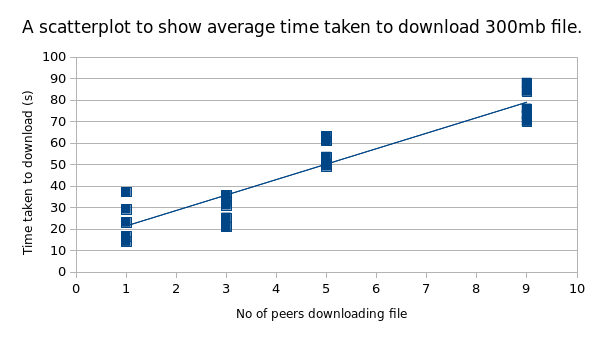
\includegraphics[scale=0.50]{images/graph.png}
\end{figure}

Another overhead is caused by my design choice to serialisation. The data is read into already allocated buffer and then serialised. More memory is allocated to store that object which is costly. 

A lock is acquired on the class for reading and writing to files. I was concerned that moving the file pointer while reading or writing between two threads would cause erroneous behaviour.

Finally, my download algorithm could use improvement, I had planned to implement choking to allow a given peer to choose which peers can download from it. This would have had immense performance gains by forcing the peer to download from a less busy peer. I believe this would have produced a logarithmic graph for a small amount of peers as well.

\begin{thebibliography}{8}
  
\bibitem{wiki} 
Wikipedia Kademlia Article  
\\\texttt{https://en.wikipedia.org/wiki/Kademlia}

\bibitem{paper} 
Kademlia Paper
\\\texttt{https://pdos.csail.mit.edu/~petar/papers/maymounkov-kademlia-lncs.pdf}

\bibitem{gleamly} 
Gleamly
\\\texttt{http://gleamly.com/article/introduction-kademlia-dht-how-it-works}

\bibitem{go1}
An example implementation in Go P1  
\\\texttt{http://blog.notdot.net/2009/11/Implementing-a-DHT-in-Go-part-1}

\bibitem{go2} 
An example implementation in Go P2
\\\texttt{http://blog.notdot.net/2009/11/Implementing-a-DHT-in-Go-part-2}

\bibitem{xlattice} 
Xlattice's specification (Available on wayback machine)
\\\texttt{http://xlattice.sourceforge.net/components/protocol/kademlia/specs.html}

\bibitem{bep5} 
Bittorent's BEP
\\\texttt{http://www.bittorrent.org/beps/bep\_0005.html}

\bibitem{theory} 
Theory Wiki
\\\texttt{https://wiki.theory.org/index.php/BitTorrentSpecification}

\end{thebibliography}


\end{document}

